% !TeX spellcheck = nl_NL
\begin{savequote}[0.55\linewidth]
	``De trein naar .. heeft een vermoedelijke vertraging van ... minuten. \#typischvlaamsezinnetjes''
	\qauthor{\textasciitilde 
		Jan Dorie @oombom}
\end{savequote}

\chapter{Inleiding}
\label{chap:intro}
Openbaar vervoer is een essentiële dienst in elke stad~\citep{programmableweb14}. Om vlot van dit openbaar vervoer gebruik te maken, zijn er tientallen websites en apps (user-agents of clients) die gebruikers informatie verstrekken over vertrekken, aankomsten, ritten, routes en vertragingen. Voorbeelden hiervan zijn iRail.be, HyperRail en Railer in België, en CityMapper, TheTransitApp, Here WeGo en Google maps wereldwijd. Op dit moment zijn al deze user-agents echter toegewezen op het gebruik van data dumps of specifieke API's om informatie met betrekking tot openbaar vervoer te publiceren, of een variant ervan. 

Enerzijds zijn er volledige data dumps, in de vorm van General Transit Feed Specification (GTFS)\footnote{https://developers.google.com/transit/gtfs/} en General Transit Feed Specification Realtime (GTFS-RT)\footnote{https://developers.google.com/transit/gtfs-realtime/}. GTFS bestanden bevatten informatie over alle voertuigen van een dienstverlener, over een relatief grote tijdspanne, typisch enkele maanden tot een jaar. GTFS-RT-bestanden bevatten realtime informatie over ritten in de komende uren tot dag. Om al deze data compact op te slaan en te versturen, worden deze opgeslagen als een verzameling regels in een database-achtige structuur, zoals te zien in figuur~\ref{fig:gtfsScheme}. Deze regels omschrijven wanneer welk voertuig welke rit maakt. Om op basis van deze regels vragen te beantwoorden, dient deze verzameling abstracte regels omgevormd te worden naar een gepast model waarin informatie over ritten en stopplaatsen opgevraagd kan worden, en routes berekend kunnen worden. Hiervoor zijn, afhankelijk van welke informatie gewenst is, zware berekeningen vereist, die afhankelijk van de grootte van het GTFS bestand vijf à tien minuten kunnen duren op een moderne computer. Gebruikers kunnen geen 10 minuten wachten tot de data getransformeerd zijn, waardoor deze optie niet beschikbaar is op mobiele toestellen. Verder is dit formaat een mogelijke technologische restrictie op de reisinformatie: enkel gevorderde ontwikkelaars kunnen hiervan gebruik maken. Open data is slechts open als deze (onder andere) beschikbaar zijn in een begrijpbaar formaat~\citep{okfn18}. GTFS is dus vooral geschikt om reisinformatie te delen met grote bedrijven, en in mindere mate voor individuele ontwikkelaars die reisinformatie eenvoudig willen visualiseren (digital signage, routeplanner applicaties, websites, ...).

\begin{figure}
	\centering
	\includegraphics[width=0.5\textwidth]{images/GTFS_scheme.pdf}
		\caption[GTFS structuur]{De bestandsstructuur van GTFS data.}
	\label{fig:gtfsScheme}
\end{figure}
 
Anderzijds zijn er traditionele Remote Procedure Call (RPC) zoals iRail\footnote{https://irail.be}, die beschikken over verschillende endpoints om specifieke vragen te beantwoorden. Bij deze API's wordt, zoals de naam reeds doet vermoeden, een procedure op de server aangeroepen. Dit is duidelijk zichtbaar in de schematische voorstelling in figuur~\ref{fig:rpcScheme}. Achterliggend kunnen zware berekeningen uitvoeren of grote databases geraadpleegd worden zonder dat de gebruiker hier nadeel van ondervindt. Deze antwoorden zijn rechtstreeks bruikbaar voor de client, maar bieden enkel het antwoord op één specifieke vraag. Om een andere vraag te beantwoorden, al dan niet gesteld door dezelfde client, is een nieuw verzoek naar de server nodig, en moet het nieuwe antwoord verwerkt worden. Voor elk verzoek naar de server is een verbinding tussen de client en server benodigd, en relatief veel processortijd van de server. Een continue internetverbinding is dus vereist, en server-side is een potentieel grote en dure infrastructuur nodig om aan alle vragen te voldoen. Een ander belangrijk nadeel bij deze techniek is dat deze data moeilijk te combineren zijn met andere datasets. Een route plannen die gebruik maakt van meerdere openbaar vervoer aanbieders is enkel mogelijk als een API beschikbaar is die achterliggend door meerdere datasets zoekt. Twee API's combineren om de beste route via meerdere vervoersmaatschappijen te vinden is niet op een eenvoudige manier mogelijk.

\begin{figure}
	\centering
	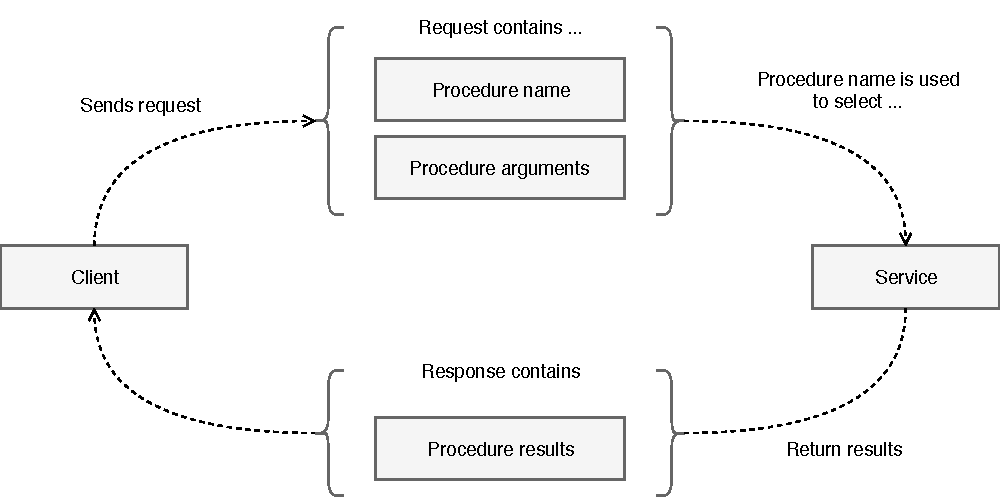
\includegraphics[width=0.80\textwidth]{rpc_api.pdf}
	\caption[RPC structuur]{De werkwijze van een RPC API.}
	\label{fig:rpcScheme}
\end{figure}

Deze twee methodes zijn elkaars tegengestelde. Ontwikkelaars moeten kiezen voor data die compact maar complex -- en slechts indirect bruikbaar -- is, of voor een vraag-antwoord systeem wat voor elke nieuwe vraag een nieuw verzoek naar een server moet maken. Aan de IDLab onderzoeksgroep aan UGent is onderzoek gedaan naar Linked Connections (LC)\footnote{https://linkedconnections.org}, een nieuw formaat dat een nieuw evenwicht tracht te vinden tussen de bestaande oplossingen. Alle vertrekken van alle voertuigen worden in één chronologische lijst verzameld, waarbij de lijst kan opgevraagd worden volgens vaste tijdsintervallen met een grootteorde van enkele minuten. Hierdoor hoeft de server enkel deze lijst in fragmenten aan te bieden, waarbij alle clients dezelfde informatie krijgen. De clients dienen zelf nog berekeningen te maken, maar deze zijn relatief eenvoudig vergeleken met de berekeningen die nodig zijn om een GTFS feed te verwerken. Data in het Linked Connections-formaat kunnen eenvoudig toegankelijk gemaakt worden via een open-source serverapplicatie\footnote{https://github.com/julianrojas87/linked-connections-server/}.

\begin{figure}
	\centering
		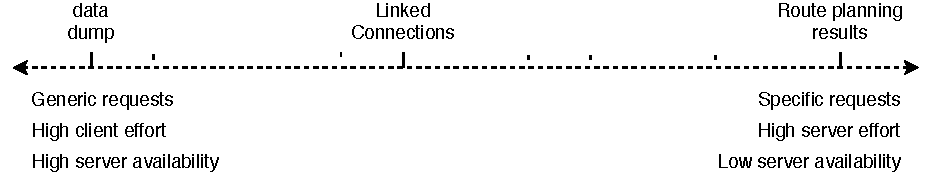
\includegraphics[width=1.0\textwidth]{ldf_axis.pdf}
	\caption[Routeplanning HTTP-interfaces op de LDF as]{De Linked Data Fragments as illustreert dat alle HTTP-interfaces data fragmenten aanbieden, maar verschillen in hoe specifiek de aangeboden data is, en dus de moeilijkheid om deze aan te maken~\citep{verborgh14}. In deze figuur is de as toegepast op HTTP-interfaces voor routeplanning~\citep{colpaert15}.}
	\label{fig:ldfAxis}
\end{figure}

\section{Wat is user-perceived performance?}
\label{sec:what_is_user_perceived_performance}
Elke interface voor het ophalen van data heeft specifieke eigenschappen zoals latency, performance, cache-hergebruik,...~\citep{verborgh16}. Wanneer we verschillende technieken vergelijken door voor elke techniek dezelfde user-agent te gebruiken, kunnen we de impact van de verschillende achterliggende technieken op de eindgebruiker onderzoeken. Hiervoor definiëren we de \foreign{user-perceived performance}. De user-perceived performance is de performance zoals de gebruiker deze ervaart, welke niet strikt gelijk hoeft te zijn aan de werkelijke performance van technische component. De user-perceived latency werd gedefinieerd in 2000 door Roy T. Fielding gedefinieerd als de tijd tussen het selecteren van een link en het renderen van een bruikbaar resultaat~\citep{fielding99}. Latency treedt volgens Fielding op verschillende punten: 
\begin{enumerate}
	\item de tijd die de client nodig heeft om actie te ondernemen 
	\item de tijd die nodig is voor voorbereidende acties
	\item de tijd om een verzoek te verzenden
	\item de tijd die de server nodig heeft om het antwoord te bepalen
	\item de tijd die nodig is om het antwoord te verzenden
	\item de tijd voor het antwoord te verwerken en weer te geven
\end{enumerate}
Terwijl enkel stappen 3, 4 en 5 rechtstreeks afhankelijk zijn van het netwerk, kunnen al deze stappen beïnvloed worden door de gebruikte techniek~\citep{fielding99}.

Wanneer we ons niet enkel op de prestaties richten, maar ook op de manier waarop de gebruiker omgaat met de technologie, komen we bij de gebruikerservaring of user-experience (UX) terecht. User-experience is een brede term, die oorspronkelijk gebruikt werd voor het ontwerp en gebruik van interfaces, waardoor het een synoniem vormde voor interacties en bruikbaarheid~\citep{avila11}. Een ander gebruik van de term focust op de niet-instrumentele noden en ervaringen in een complexere zin~\citep{avila11}. In beide gevallen is UX een centraal belang in Human-Computer Interfaces (HCI)~\citep{NíChonchúir2008}. In deze masterproef zullen we de user-experience steeds in deze bredere zin beschouwen. 

Ondertussen zijn we geëvolueerd naar een wereld waarin data vaak mobiel geconsumeerd worden: 78\% van de Vlamingen beschikt over een smartphone, 80,5\% beschikt over een laptop. Slechts 41,8\% beschikt over een desktop-computer~\citep{digimeter17}. Bij deze mobiele toestellen zijn er ook andere aspecten die meespelen in de user-experience: batterijgebruik en offline toegang tot data vormen een aanzienlijke factor~\citep{ickin12}. Een applicatie biedt een betere ervaring wanneer deze dezelfde data kan weergeven met aanzienlijk minder energieverbruik, of wanneer deze consistent goed presteert, ook wanneer netwerk slecht of niet beschikbaar is. Hoewel de user-perceived performance een groot belang heeft in de user-experience van een applicatie, dienen we dus ook deze andere aspecten in rekening te brengen. Mobiele gebruikers hebben ook nog steeds angst om te veel data te verbruiken~\citep{ammelrooy17}.

% TODO: zal dit zo blijven of is er een trend ivm angst over datalimiet?

\section{Probleemstelling en doel van de masterproef}
\label{sec:problem}

Linked Connections werd ontwikkeld met de bedoeling een evenwicht te vinden tussen data dumps en RPC API's. In plaats van elke query op een server te beantwoorden, wordt een gelinkte lijst van connecties gepubliceerd. Linked Connections laat hierdoor toe om vragen te beantwoorden door middel van een lineair groeiende lijst van connecties te overlopen~\citep{colpaert15}. Bovendien gebruiken alle user-agents dezelfde lijst, waardoor deze zeer cachebaar is. Bij stijgende belasting daalt de tijd die de server nodig heeft per verzoek~\citep{colpaert17}.

Terwijl de cost-efficiency van Linked Connections reeds is aangetoond, waarbij Linked Connections hetzelfde aantal verzoeken kan beantwoorden met slechts 25\% van de rekencapacteit~\citep{colpaert17,Melendez17}, is er nog geen onderzoek gebeurt naar de user-perceived performance van een user-agent wanneer deze gebruik maakt van Linked Connections, vergeleken met wanneer deze zelfde user-agent gebruik maakt van een traditionele RPC API. 

In deze studie richten we ons specifiek op routeplanning gebruik makend van mobiele toestellen. Deze toestellen hebben minder processorkracht en geheugen vergeleken met traditionele computers, maar ook bandbreedte en beschikbaarheid van internet zijn vaak beperkt. In het slechtste geval is er geen netwerkverbinding, waarbij enkel een cache beschikbaar is. Verder zullen we ons specifiek richten op het verschil tussen een RPC API gebaseerd op Linked Connections~\citep{colpaert17} en de originele Linked Connections webserver. Als user-agent zullen we een \foreign{fork} van de HyperRail\footnote{https://hyperrail.be} applicatie voor Android gebruiken, gemodificeerd om gebruik te maken van de genoemde API's. Door deze testopstelling zijn de oorspronkelijke data, de server hardware, de user-agent en de client hardware identiek bij elke vergelijking. Enkel het formaat voor serverinteracties en transport van data zal verschillen.

Om routes te berekenen zullen we gebruik maken van het Connection Scan Algorithm (CSA)~\citep{strasser13,strasser14,strasser17}. Dit algoritme vereist een op vertrektijd gesorteerde lijst van vertrekken. Dit is de exacte definitie van de Linked Connections knowledge graph, waardoor dit algoritme zonder al te veel modificaties toegepast kan worden. Fragmenten kunnen hierbij geladen worden op het moment dat ze nodig zijn. We zullen dezelfde implementatie gebruiken zowel bij de client-side API als bij de server-side API om zo correct mogelijke resultaten te behalen. 

In eerste instantie zal een traditionele (RPC) API geschreven worden welke gebruik maakt van de Linked Connections fragmenten op de Solid State Disk (SSD) van de server. Deze API zal endpoints bevatten voor het tonen van vertrekken en aankomsten per station, het berekenen van routes, en voor het weergeven van het traject per trein. 
Vervolgens zal een API zonder specifieke server-side geïmplementeerd worden in de applicatie. Deze zal dezelfde informatie ter beschikking stellen in de applicatie, maar zal hiervoor enkel (delen van) de gelinkte lijst met vertrekken downloaden. 

Eenmaal beide API's volledig geïmplementeerd zijn, zal de user-perceived performance onderzocht worden. Hiertoe worden begeleide user tests gehouden, waarbij een aantal testers afwisselend met beide API's hun dagelijkse opzoekingen zullen uitvoeren, waarna ze aan de hand van een vragenlijst bevraagd zullen worden naar hun ervaringen en voorkeuren. Het is essentieel om de subjectieve ervaringen van gebruikers te bevragen, gezien verschillende gebruikers mogelijk verschillende afwegingen maken. We verwachten dat sommige gebruikers offline toegang waardevol zullen vinden, terwijl anderen mogelijk geen belang hechten aan offline toegang. Ook zal getracht worden technische data te verzamelen, zoals geheugen- en processorgebruik, laadtijden, en batterijverbruik. 

Deze masterproef zal gebruik maken van data afkomstig van de NMBS om routeplanning en realtime data over treinen in België weer te geven. Door de bron van de data te vervangen kan dit onderzoek ook toegepast worden op andere openbaar vervoer maatschappijen die gebruik maken van tijdsschema's, ongeacht het soort voertuig dat gebruikt wordt.

\section{Onderzoeksvraag}
 \label{sec:onderzoeksvraag}
 
Zoals in de vorige sectie werd besproken, zullen we onderzoeken welke API de beste gebruikerservaring oplevert. Dit formuleren we nu in een onderzoeksvraag, die we zullen beantwoorden in hoofdstuk~\ref{chap:interpretatie}.
 
\paragraph{Onderzoeksvraag} Verbetert de user-experience en user-perceived performance van een applicatie voor openbaar vervoer wanneer gebruik gemaakt wordt van Linked Connections in plaats van traditionele RPC API's?
 
Regelmatig klagen mensen over de kwaliteit van hun netwerkverbinding bij treinreizen. Hierbij klaagt men over een trage of afwezige verbinding. We vermoeden dat de gebruiker hierdoor gehinderd wordt bij het online opzoeken van informatie, en liefst op elk moment van zijn treinreis over reisinformatie wilt kunnen beschikken, ongeacht de kwaliteit van het mobiele netwerk.
\paragraph{Hypothese 1} Gebruikers beschikken niet over een kwalitatieve internetverbinding tijdens het reizen, en ervaren de mogelijkheid voor offline zoekopdrachten als een meerwaarde.
 
Uit gesprekken met treinreizigers blijkt dat een aantal reizigers snellere routes kent dan de routes die applicaties op basis van officiële data voorstellen. Zo kan een lange overstap worden voorkomen door zich te haasten bij het overstappen. We vermoeden dat gebruikers het handig vinden om deze routes ook in hun routeplanning applicatie kunnen terug te vinden. We vermoeden ook dat minder mobiele gebruikers graag beperkingen zouden kunnen stellen aan de route, om bijvoorbeeld niet over te stappen in stations zonder verhoogde perrons.
\paragraph{Hypothese 2} De gebruiker ervaart de mogelijkheid om voorkeuren voor routes in te stellen (overstaptijd, toegankelijkheid, ...) als een meerwaarde.
 
Zoals eerder vermeld hebben mobiele gebruikers ook nog steeds angst om te veel data te verbruiken~\citep{ammelrooy17}. We vermoeden dat dit ook nog steeds zo is, maar dit geen zorg is van gebruikers wanneer ze applicaties voor openbaar vervoer gebruiken.
\paragraph{Hypothese 3} De gebruiker heeft angst om te veel mobiele data te verbruiken, maar let hier niet op bij het gebruik van routeplanning-apps.
 
Hoewel privacy een \foreign{hot topic} is, vermoeden we dat de modale treinreiziger geen belang hecht aan zijn of haar privacy bij het gebruik van routeplanning applicaties. We vermoeden dat de gebruiker extra privacy als positief ervaart, maar zijn keuze voor een routeplanning applicatie hier niet door laat beïnvloeden.
\paragraph{Hypothese 4} De gebruiker ervaart extra privacy bij het opzoeken van routes niet als een noemenswaardige meerwaarde